\chapter{ Аналитический раздел}
\label{cha:analysis}

Lorem ipsum dolor sit amet, consectetur adipiscing elit. Integer a mauris consequat, sagittis odio ut, tempor lacus. Donec rhoncus tincidunt ligula, vel egestas turpis vehicula interdum. Phasellus sit amet dignissim metus, quis rutrum metus. Nullam euismod dictum rhoncus. Vivamus bibendum gravida lacus, iaculis consectetur nunc suscipit ac. Aliquam erat volutpat. Nulla laoreet, elit vel lacinia egestas, metus erat sagittis orci, quis vulputate urna tellus ut felis. Morbi sit amet elit auctor, ultrices dui eu, elementum nisi.



\section{Теория цвета}
Прежде всего, необходимо разобраться с тем, что такое цвет. Цвет -- это воприятие волн определённого рода электромагнитной энергии, которые после восприятия глазом и мозгом человека преобразуются в цветовые ощущения. Видимый человеком цвет возникает, с одной стороны, под влиянием объективного физического явления — света, с другой — в результате электромагнитного излучения различных частот на зрительный аппарат человека. Помимо этих факторов, на возникновение цветового ощущения человека влияют зрительный опыт и память, физиологические и психологические особенности.

\subsection{Трёхкомпонентная теория цветовосприятия}
Трёхкомпонентная теория цветовосприятия — теория, объясняющая цветовое зрение человека, основанное на восприятие трех основных компонентов цвета. Из научных опытов было обнаружено, что в сетчатке глаза человека есть три вида колбочек, максимумы чувствительности которых приходятся на красный, зелёный и синий участки спектра. \cite{b1}  Трёхсоставную теорию цветового зрения впервые высказал в 1756 году М. В. Ломоносов, когда он писал «о трёх материях дна ока». Сто лет спустя её развили немецкий и английский учёные Г. Гельмгольц и Т. Юнг. Параллельно существовала оппонентная теория цвета Эвальда Геринга, которая предполагла что в мозг поступает информацию о разнице яркости — о разнице яркости белого и чёрного, о разнице зелёного и красного цветов, о разнице синего и жёлтого цветов, где жёлтый цвет есть сумма красного и зелёного цветов.  На теории о трёх составляющих цвета и строится большинство цветовых моделей. 

\subsection {Цветовые пространства и модели}
Цветовая модель -- это способ представления цвета в виде кортежа некоторых его независимых между собой] характеристик. Как правило, это три составляющие его компоненты, например красный, зелёный и синий или тон, насыщенность и яркость. Цветовое пространство же -- это представление цветового множества с помощью осей координат, где каждая ось преставляет возможные значения одной из компонент кортежа из цветовой модели. 

\subsubsection{RGB}

\subsubsection{XYZ}
Это — эталонная цветовая модель, заданная в строгом математическом смысле организацией CIE (Commission Internationale de l'Éclairage— Международная комиссия по освещению) в 1931 году. Модель CIE XYZ является мастер-моделью практически всех остальных цветовых моделей, используемых в технических областях. В её основе лежит суждение о том, что смешение двух и более цветов можно представить как сложение соответсвующих векторов. Система CIE XYZ создана путём математических трансформаций системы CIE RGB и базируется на тех же принципах — любой цвет можно точно специфицировать количеством трёх излучений, смесь которых воспринимается человеком идентичной по цвету.



\begin{figure}[ht!]
	\centering{ 
	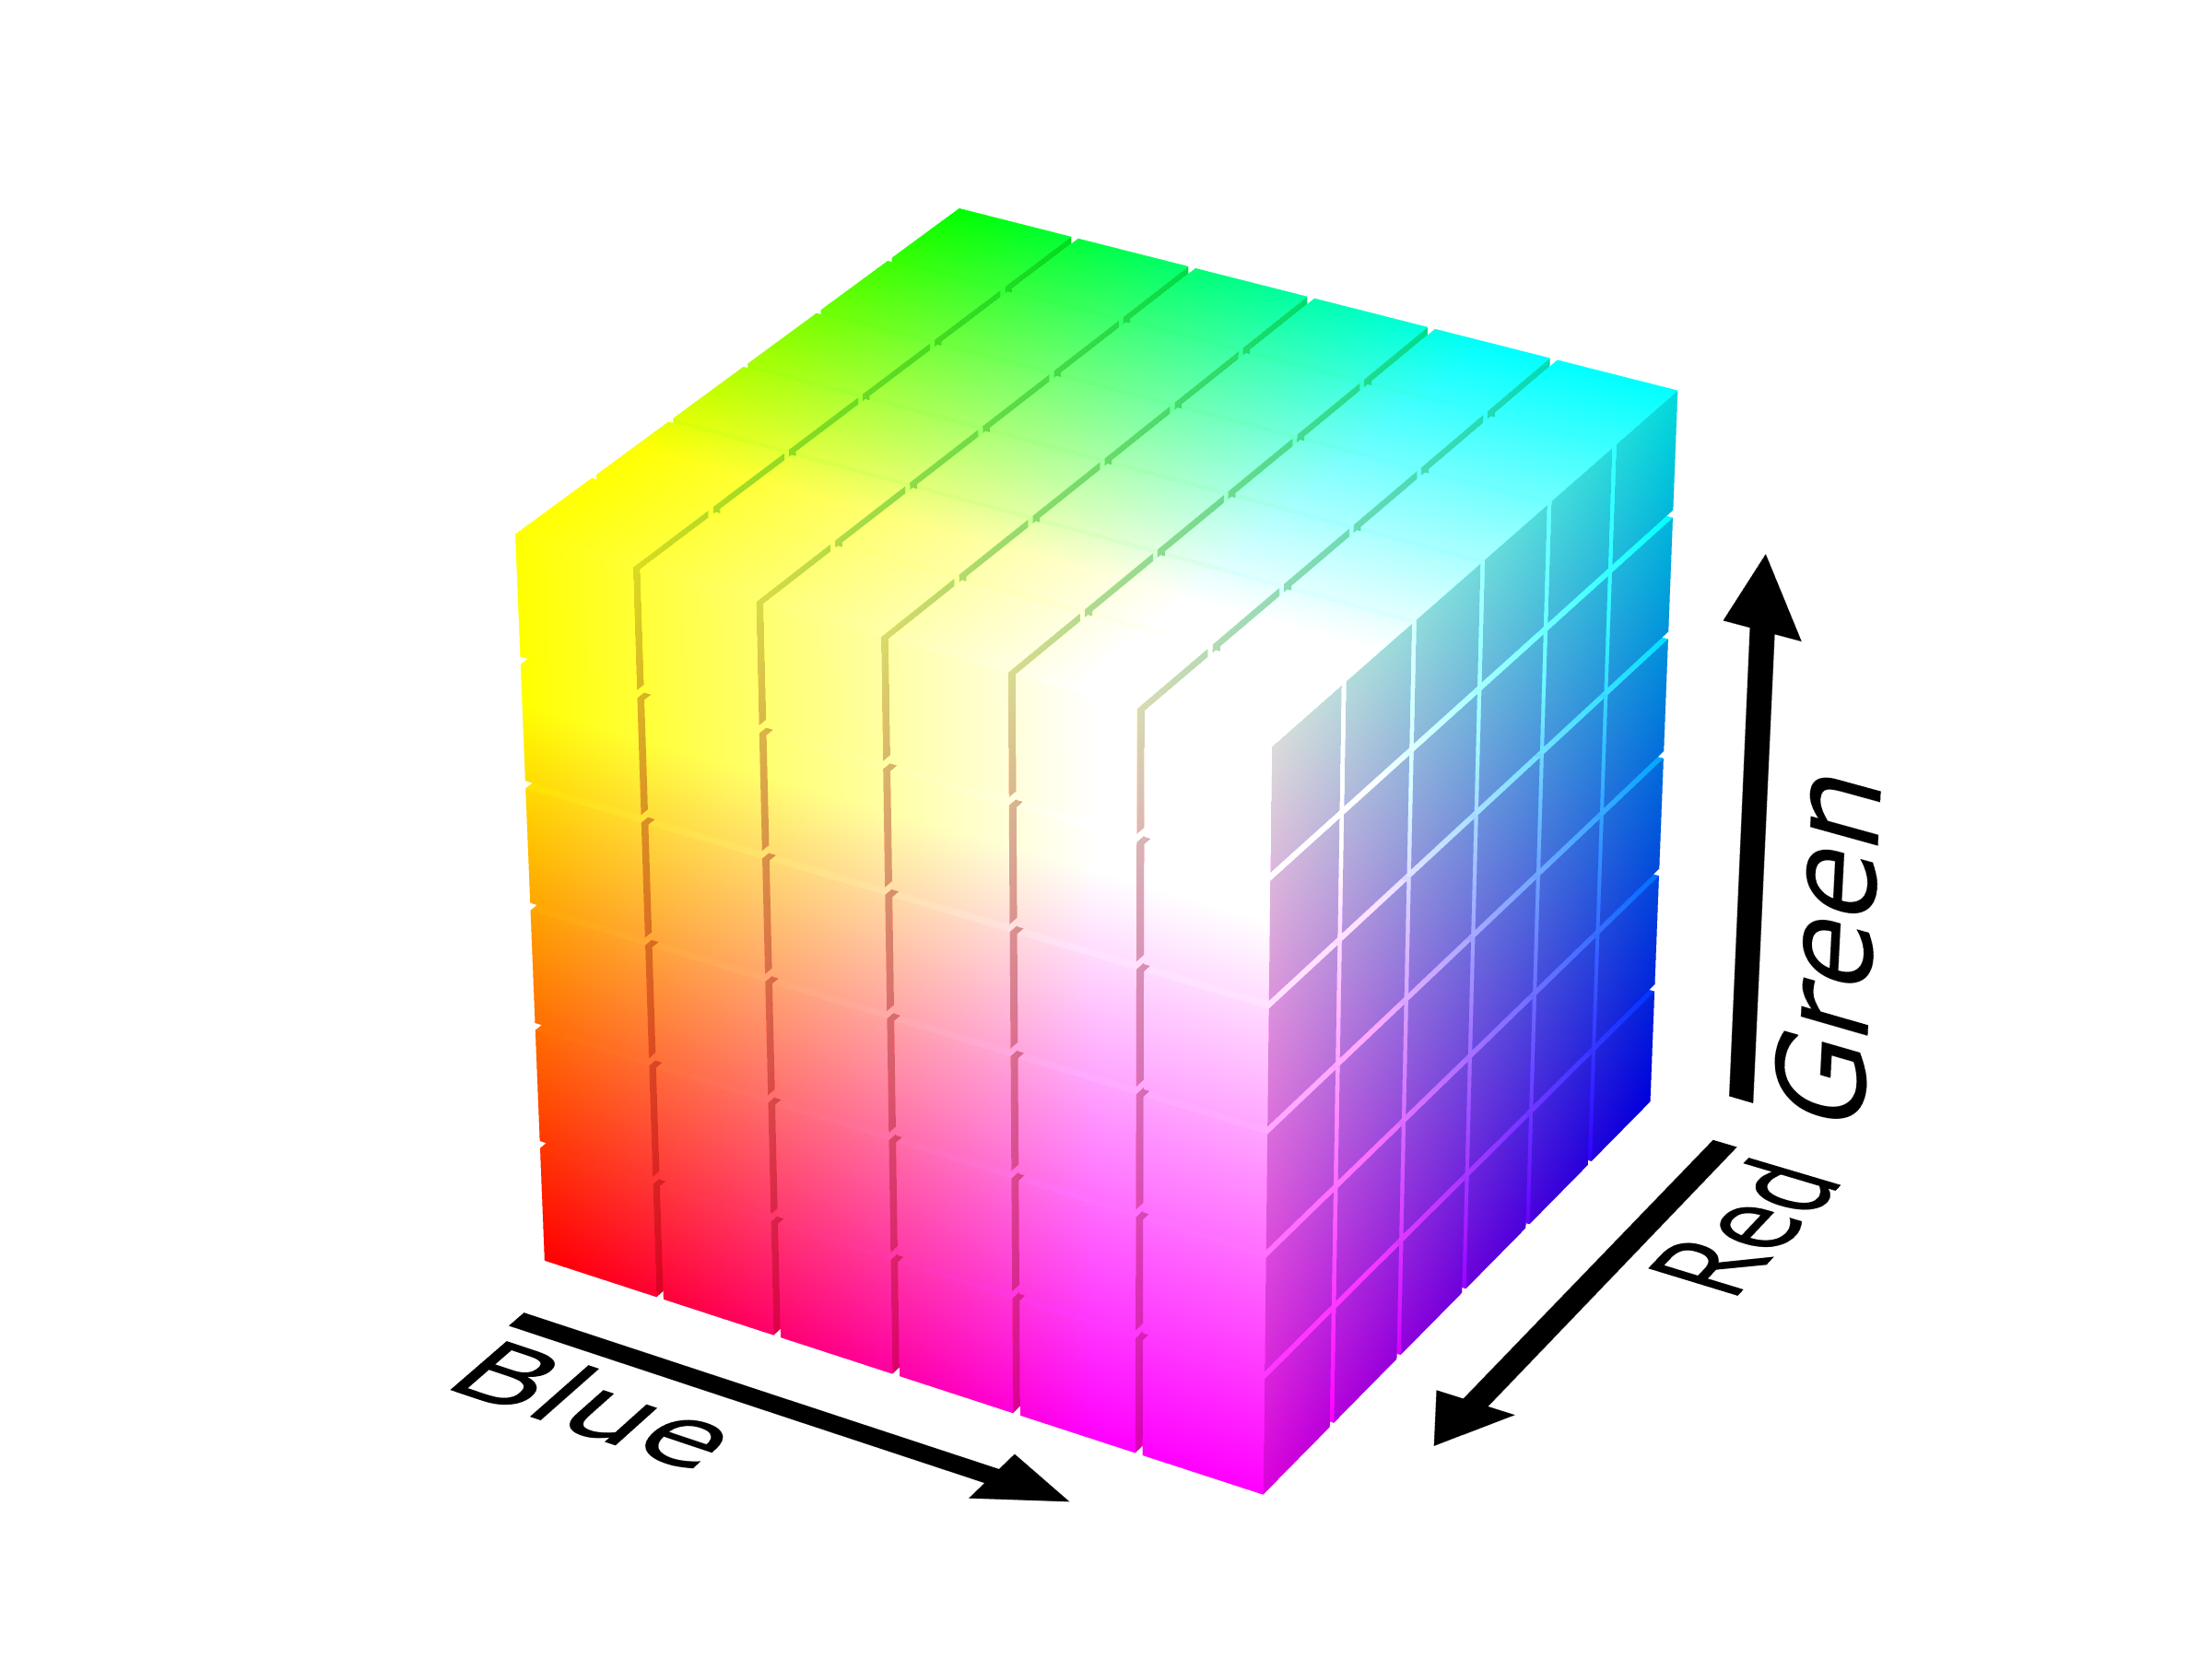
\includegraphics[width=0.4\textwidth]{img/img1.png}
	\caption{Представление цветового куба}}
\end{figure}

 Основное отличие системы XYZ — цвет её основных «излучений» существует только в колориметрических уравнениях, и получить их физически невозможно.
Основная причина создания системы XYZ — облегчения расчётов. Координаты цвета и цветности всех возможных световых излучений будут положительными. Также, координата цвета Y выражает фотометрическую яркость стимула непосредственно.
\subsubsection{CMYK}

\subsubsection{Другие цветовые модели}
\subsection{Методы смешивания цветов}
\subsubsection{Аддитивный синтез}
\subsubsection{Субтрактивный синтез}
\subsection{Альфа-канал}

\section{Альфа-смешение}

\subsection{Расчёт результирующего цвета}

\subsection{Анализ  алгоритмов смешения цветов}
\subsection{}
\section{Оптимизация вычислений}
\subsection{Анализ существующих технологии оптимизации вычисления}
\subsubsection{Технология SSE}
\subsubsection{gpu}
\subsubsection{аналитика}
\subsection{Технология AVX}
\subsubsection{Различия AVX и AVX2}
\subsubsection{Необходимые условия использования технологии AVX2}
\subsubsection{Применение AVX2 для оптимизации смешения цветов}
\subsubsection{Достоинства технологии}
\subsubsection{Недостатки технолгии}
\subsection{Сравнение возможных технологий}
\subsection{}



\begin{figure}[ht!]
	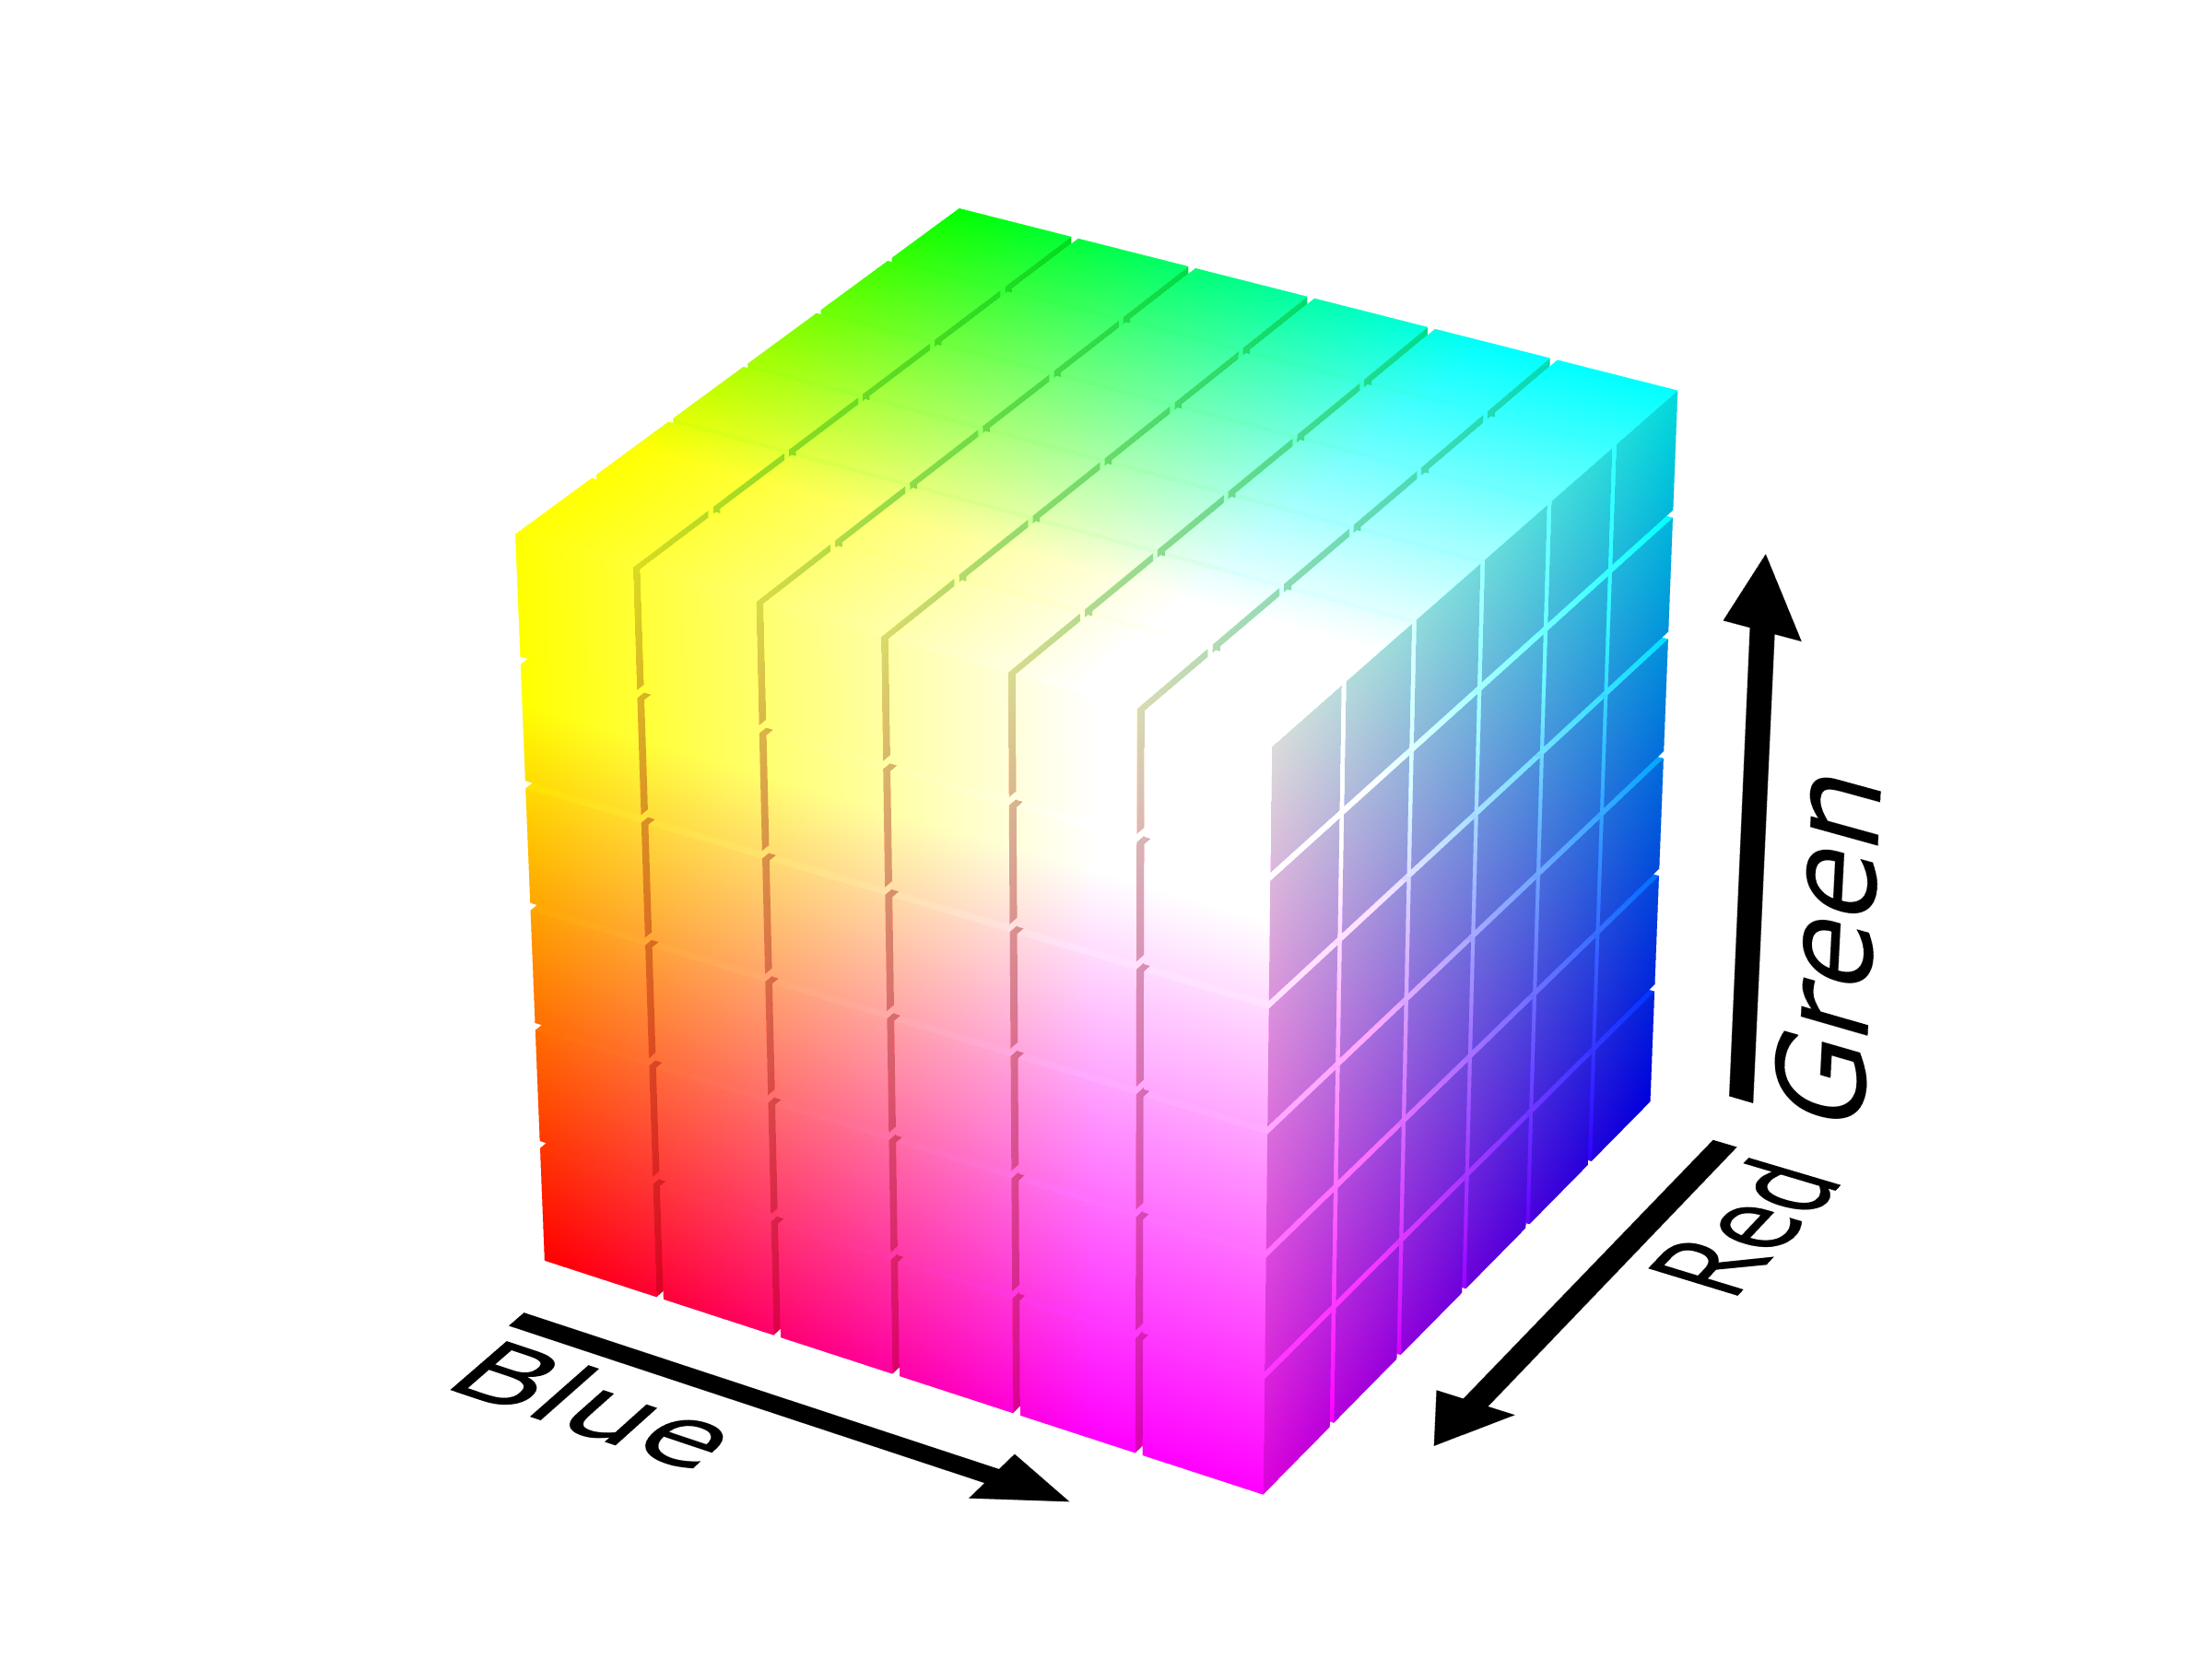
\includegraphics[width=0.4\textwidth]{img/img1.png}
	\caption{Lorem ipsum dolor sit amet}
	\label{fig:spire05}
\end{figure}


\begin{equation}
S_{p0}=\frac{T_{0} }{T_{p}} \\
\label{F:100}
\end{equation}
\begin{equation}
S_{p}=\frac{T_{1} }{T_{p}}
\label{F:101}
\end{equation}
где $T_{0}$ -- Lorem ipsum dolor sit amet, $T_{1}$ -- Lorem ipsum dolor sit amet, $T_{p}$ -- Lorem ipsum dolor sit ametLorem ipsum dolor sit amet \cite{b1}. 

Lorem ipsum dolor sit amet
\begin{equation}
1\leq S_{p} \leq p,\; \;  \frac{1}{p} \leq E_{p} \leq 1
\label{F:103}
\end{equation}



\begin{table}[h!]
	\caption{\label{tab:tbl1}Формат записи трассы PICL}
	\begin{tabular}{|l|l|}
		%	&\makebox[3em]{6/3}&\makebox[3em]{6/4}
		\hline
		Наименование поля & Назначение \\
		\hline\hline
		тип записи&тип информации в записи
		\\\hline
		тип события &тип события, с которым связана запись
		\\\hline
		отметка времени&когда информация была истинной\\\hline
		идентификатор процессора
		&процессор, с которым связана информация
		\\\hline
		идентификатор процесса	
		&процесс, с которым связана информация	
		\\\hline
		количество полей данных	
		&количество дополнительных полей данных, связанных \tabularnewline & с данными типами записи и события	
		\\\hline
		дескриптор данных	
		&формат полей данных
		\\\hline
		данные	
		&дополнительные поля данных
		\\\hline
		
	\end{tabular}
\end{table}

%%% Local Variables:
%%% mode: latex
%%% TeX-master: "rpz"
%%% End:
